\section{Stavba Země}

\subsection{Zemský plášť a kůra}
Země se sestává ze tří hlavních částí: \textbf{zemského jádra}, \textbf{pláště} a \textbf{kůry} (Obr. \ref{fig:stavba_zeme}). Hranice mezi jednotlivými částmi byly zjištěné studiem průchodu zemětřesných vln zemským tělesem. Na těchto hranicích se totiž výrazně mění chování zemětřesných vln či skrz hranici nemohou prostupovat. Rozhraní mezi zemskou kůrou a pláštěm tvoří Mohorovičičova diskontinuita (zkráceně Moho). Pod kontinenty se nachází v průměrné hloubce 35 km, pod oceány v pouhých 5--10 km pod oceánským dnem. Zemská kůra tedy nemá všude stejnou tloušťku. Mocnost \textbf{Oceánské kůry} je 5--10 km. Skládá se hlavně z bazaltové a tenké sedimentární vrstvy. \textbf{Kontinentální kůra} je daleko mocnější, v průměru má okolo 35 km avšak pod některými pohořími může dosahovat i 70 km. 

%
%\begin{myboxgreen}
%	Obrázek o stavbě Země máme díky sledování průběhu zemětřesných vln zemským tělesem.
%\end{myboxgreen}

\begin{figure*}[h]
	\includegraphics[width = \textwidth]{./tectonic/Earth_cutaway_schematic-en.pdf}
	\caption{Průřez Zemí (není v měřítku) (zdroj: USGS, volné dílo, via Wikimedia Commons)}
	\label{fig:stavba_zeme}
\end{figure*}

\subsection{Teorie deskové tektoniky}
Procesy, které ovlivňují reliéf v globálním měřítku se odehrávají v \textbf{litosféře} neboli pevném obalu Země. Litosféra je tvořena rigidními, neroztavenými horninami a zahrnuje zemskou kůru, tak i svrchní, pevnou část zemského pláště. Podle typu zemské kůry tak rozlišujeme i litosféru na oceánskou a kontinentální. 
Pod litosférou se nachází \textbf{astenosféra}. Jedná se o zónu částečně natavených hornin, což způsobuje, že se astenosféra chová plasticky. 
Litosféra není celistvá. Ve skutečnosti je rozčleněna do \textbf{litosférických desek}, které se nezávisle na sobě pohybují, po astenosféře. Existuje 7 hlavních, celá řada menších litosférických desek. Mezi ty hlavní patří Euroasijská, Pacifická, Severoamerická, Jihoamerická, Africká, Indo-australská a Antarktická. Z menších desek jsou nejznámější např. Nazca, Kokosová, Filipínská, Arabská. 

\begin{figure*}[h]
	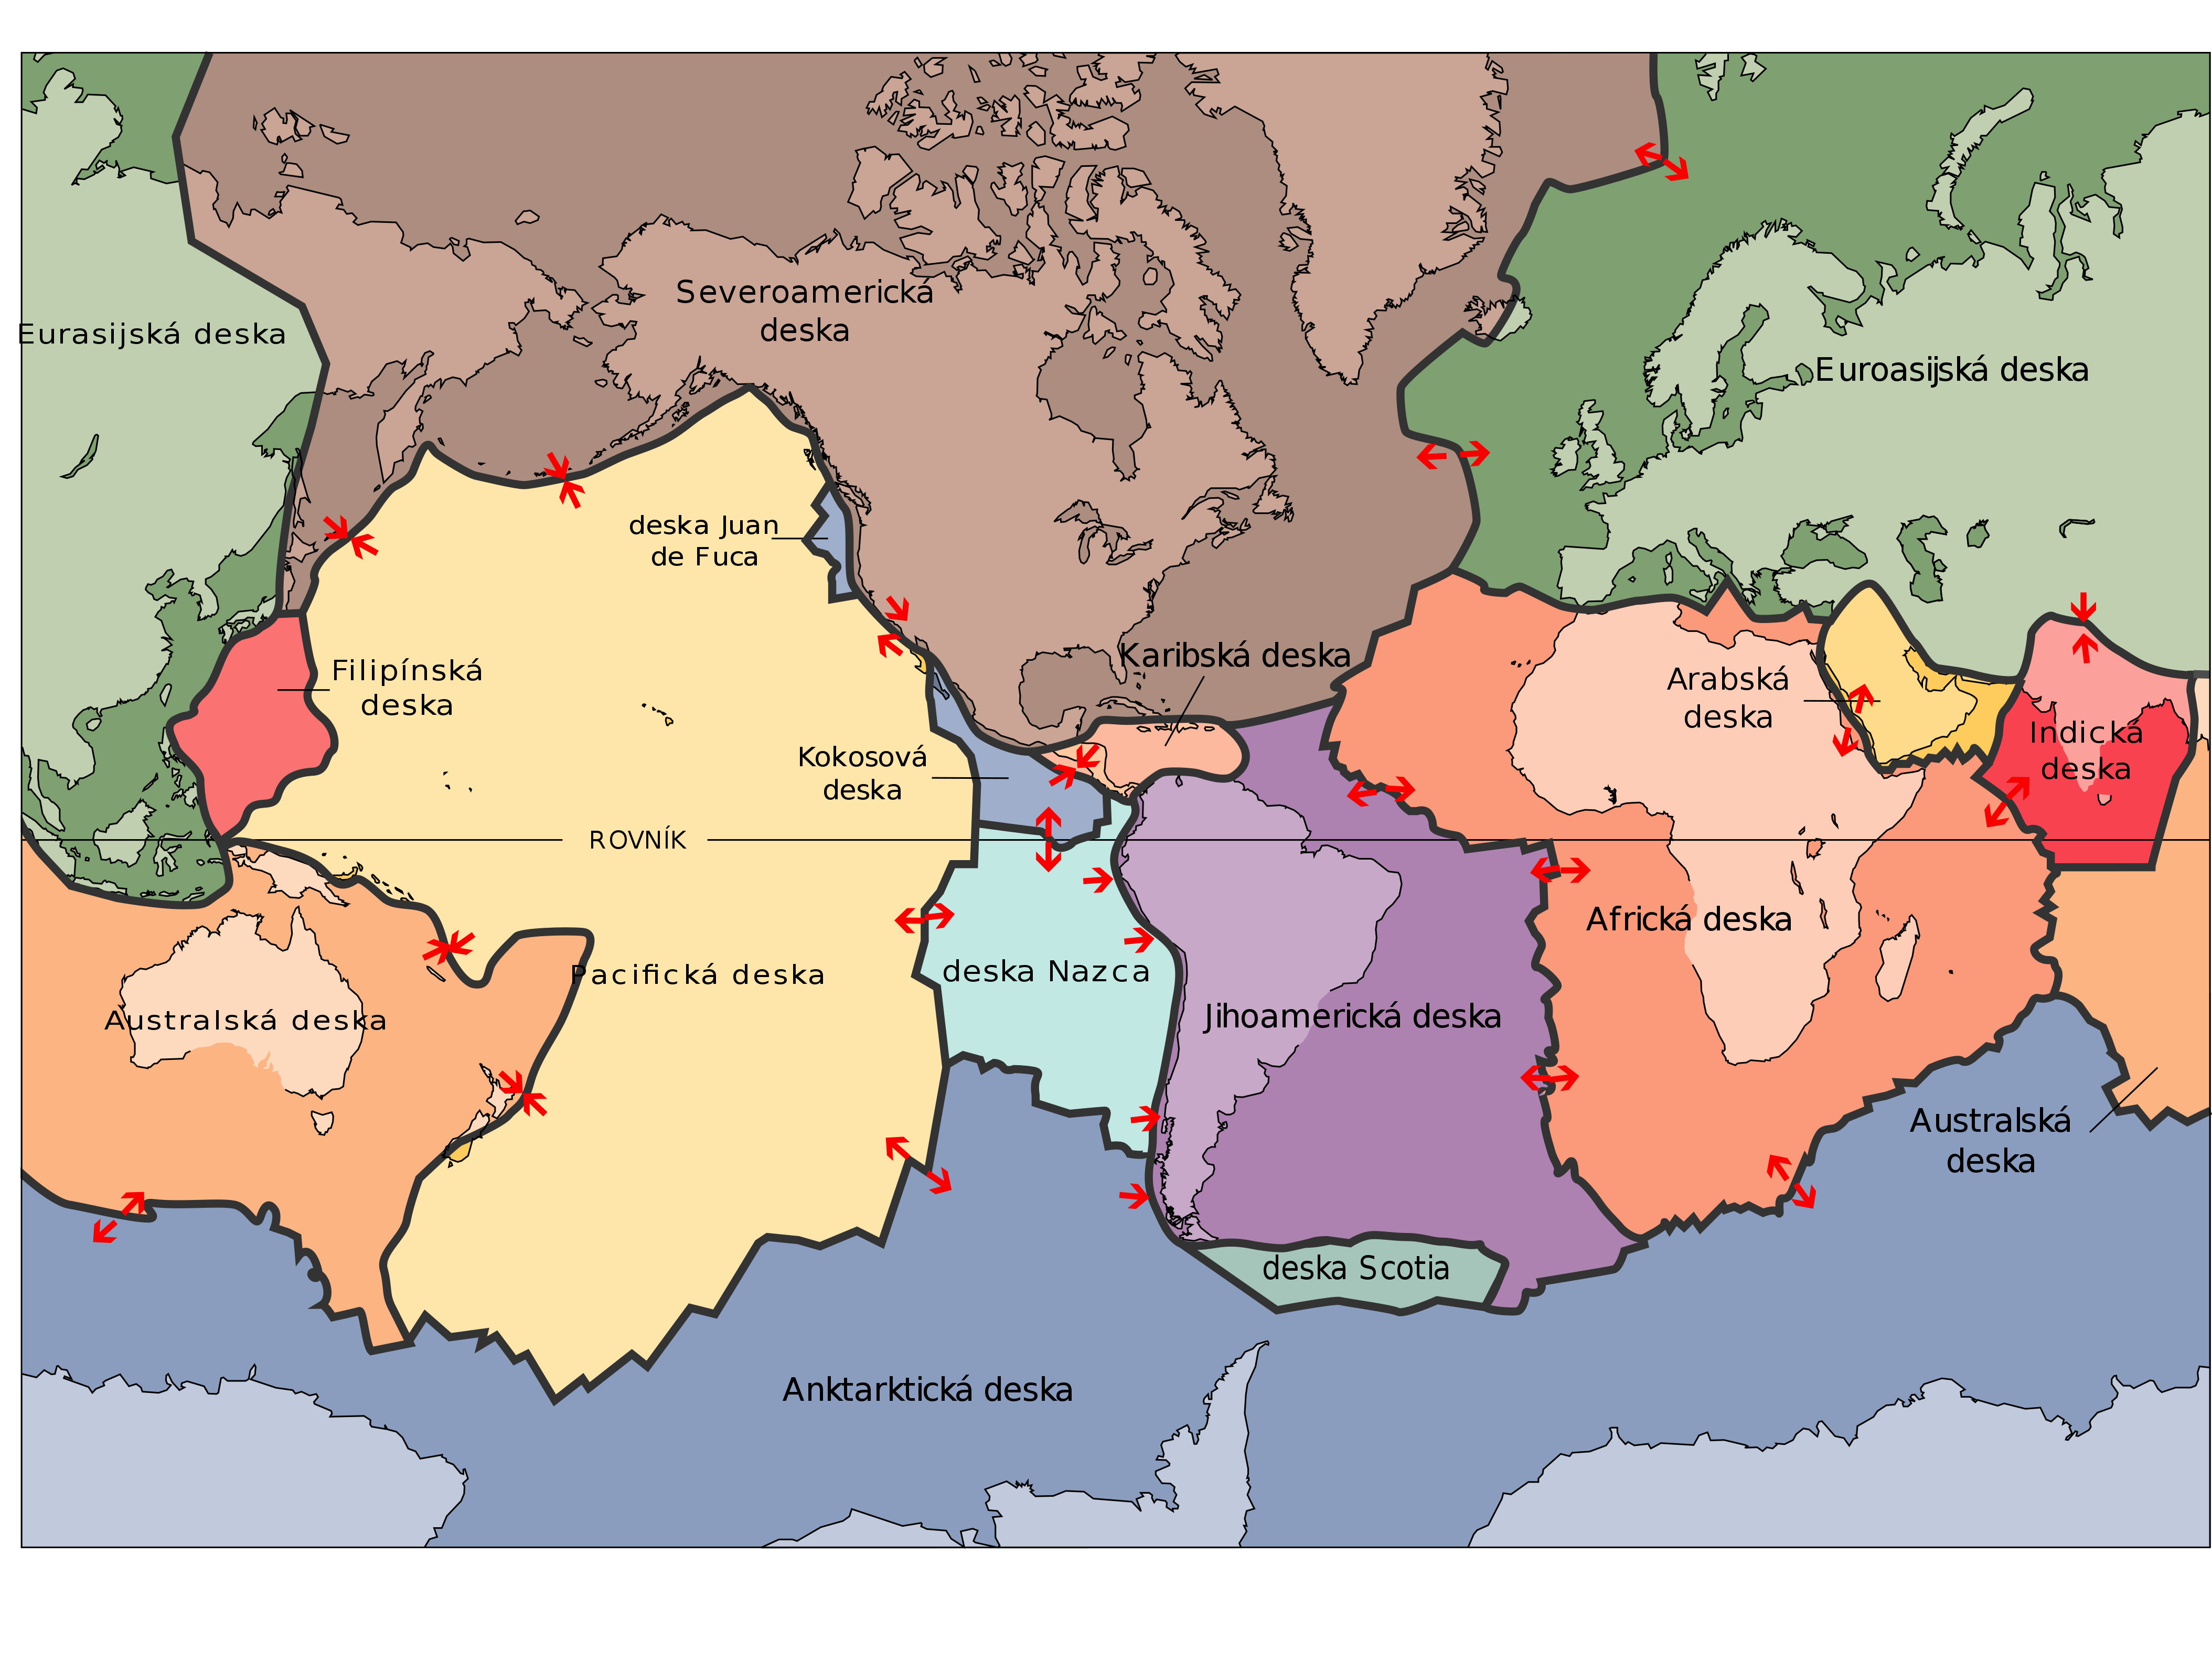
\includegraphics[width=\textwidth]{./tectonic/Plates_tect_cs.svg}
	\caption{Hlavní tektonické desky (zdroj: Jklamo, volné dílo, via Wikimedia Commons}
\end{figure*}

\subsubsection{Okraje litosférických desek}
Existují celkem tři typy rozhraní litosférických desek, a to divergentní, konvergentní a transformní. \textbf{Divergentní} rozhraní jsou takové, kde se litosférické desky od sebe vzdalují. Typickou ukázkou divergentního rozhraní jsou středooceánské hřbety jako je např. Středoatlantský hřbet. Na středooceánských hřbetech vzniká nová oceánská kůra, rozšiřuje se tak oceánské dno. Stáří oceánské kůry roste na obě strany od osy hřbetu. Středooceánské hřbety jsou rozčleněny transformními zlomy, které způsobují jejich klikatění v půdorysu. 

Při pohybu litosférických desek proti sobě hovoříme o \textbf{konvergentním} okraji. Pokud se střetávají dvě oceánské desky, jedna se podsouvá pod druhou neboli dochází k \textbf{subdukci}. V místě subdukce vzniká hlubokoceánský příkop a vulkanický ostrovní oblouk.  Subdukce oceánské litosféry pod kontinentální je opět charakteristické hlubokooceánským příkopem a dochází k orogenezi s aktivním vulkanismem. Typickým příkladem je podsouvání desky Nazca pod Jihoamerickou desku. Kde takto vznikly Andy. Při střetu dvou pevninských desek nedochází k podsouvání jedné pod druhou, nýbrž dochází k intenzivní orogenezi. 

Třetím typem je \textbf{transformní okraj} někdy také \textbf{konzervační okraj}. V tomto případě se litosférické desky pohybují horizontálně podél rozhraní. Typickým příkladem transformního okraje je zlom San Andreas.

V případě, že se okraj kontinentu shoduje s okrajem litosférické desky nazýváme ho \textbf{aktivním okrajem}. Typickým příkladem je západní okraj Jižní Ameriky. Pokud je okraj kontinentu uvnitř litosférické desky, jedná se o \emph{pasivní okraj} kontinentu. 
% TODO: \usepackage{graphicx} required
\begin{figure*}[h]
	\centering
	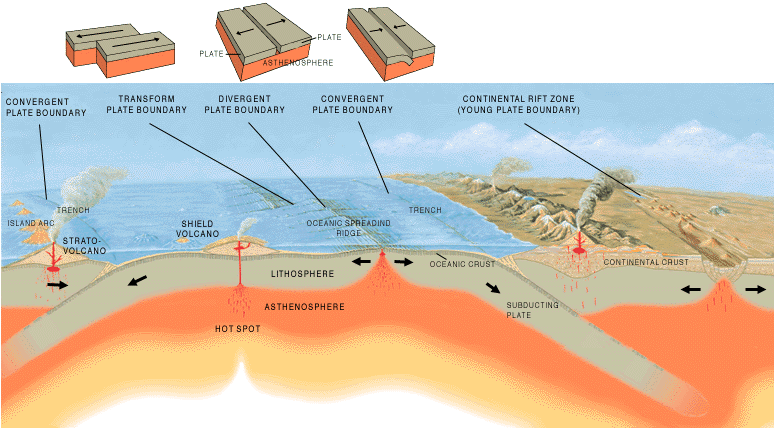
\includegraphics[width=1\linewidth]{obrazky/tectonic/Tectonic_plate_boundaries}
	\caption{Okraje litosférických desek (Autor: Jose F. Vigil. USGS, volné dílo, via Wikimedia Commons)}
	\label{fig:tectonicplateboundaries}
\end{figure*}


\begin{table*}[]
	\begin{tabularx}{1\textwidth}{XXXXXX}
		\toprule
		&          & \multicolumn{3}{c}{Morfologické a strukturní prvky}                                                                   \\ \midrule
		Typ rozhraní &
		Napěťový režim &
		Oceánská--oceánská litosféra &
		Oceánská--kontinentální litosféra &
		Kontinentální--kontinentální litosféra \\ \midrule
		Divergentní & Extenzní & Středooceánský hřbet, vulkanická aktivita & --                          & Riftová údolí, vulkanismus                  \\ \midrule
		\multirow{2}{*}{Konvergentní} &
		\multirow{2}{*}{Kompresní} &
		Oceánský příkop a vulkanický ostrovní oblouk &
		Oceánský příkop, pásemná pohoří na okrajích kontinenů a vulkanismus &
		-- \\
		&          & Komplexní kolizní zóna ostrovních oblouků & Modifikovaná pásemná pohoří & Pásemná pohoří, omezená vulkanická aktivita \\ \midrule
		Transformní & Střižný  & Hřbety a údolí                            & --                          & Zlomová zóna, bez vulkanismu               \\ \bottomrule
	\end{tabularx}
	\caption{Klasifikace a hlavní charakteristiky rozhraní litosférických desek}
	\label{tab:my-table}
\end{table*}

Okraje litosférických desek jsou důležitým místem, kde se odehrává celá řada geodynamických procesů. Jsou to místa, kde je soustředěná vulkanická a zemětřesná činnost (Obr. \ref{fig:zemetresenidesky}). 

\begin{figure*}[h]
	\centering
	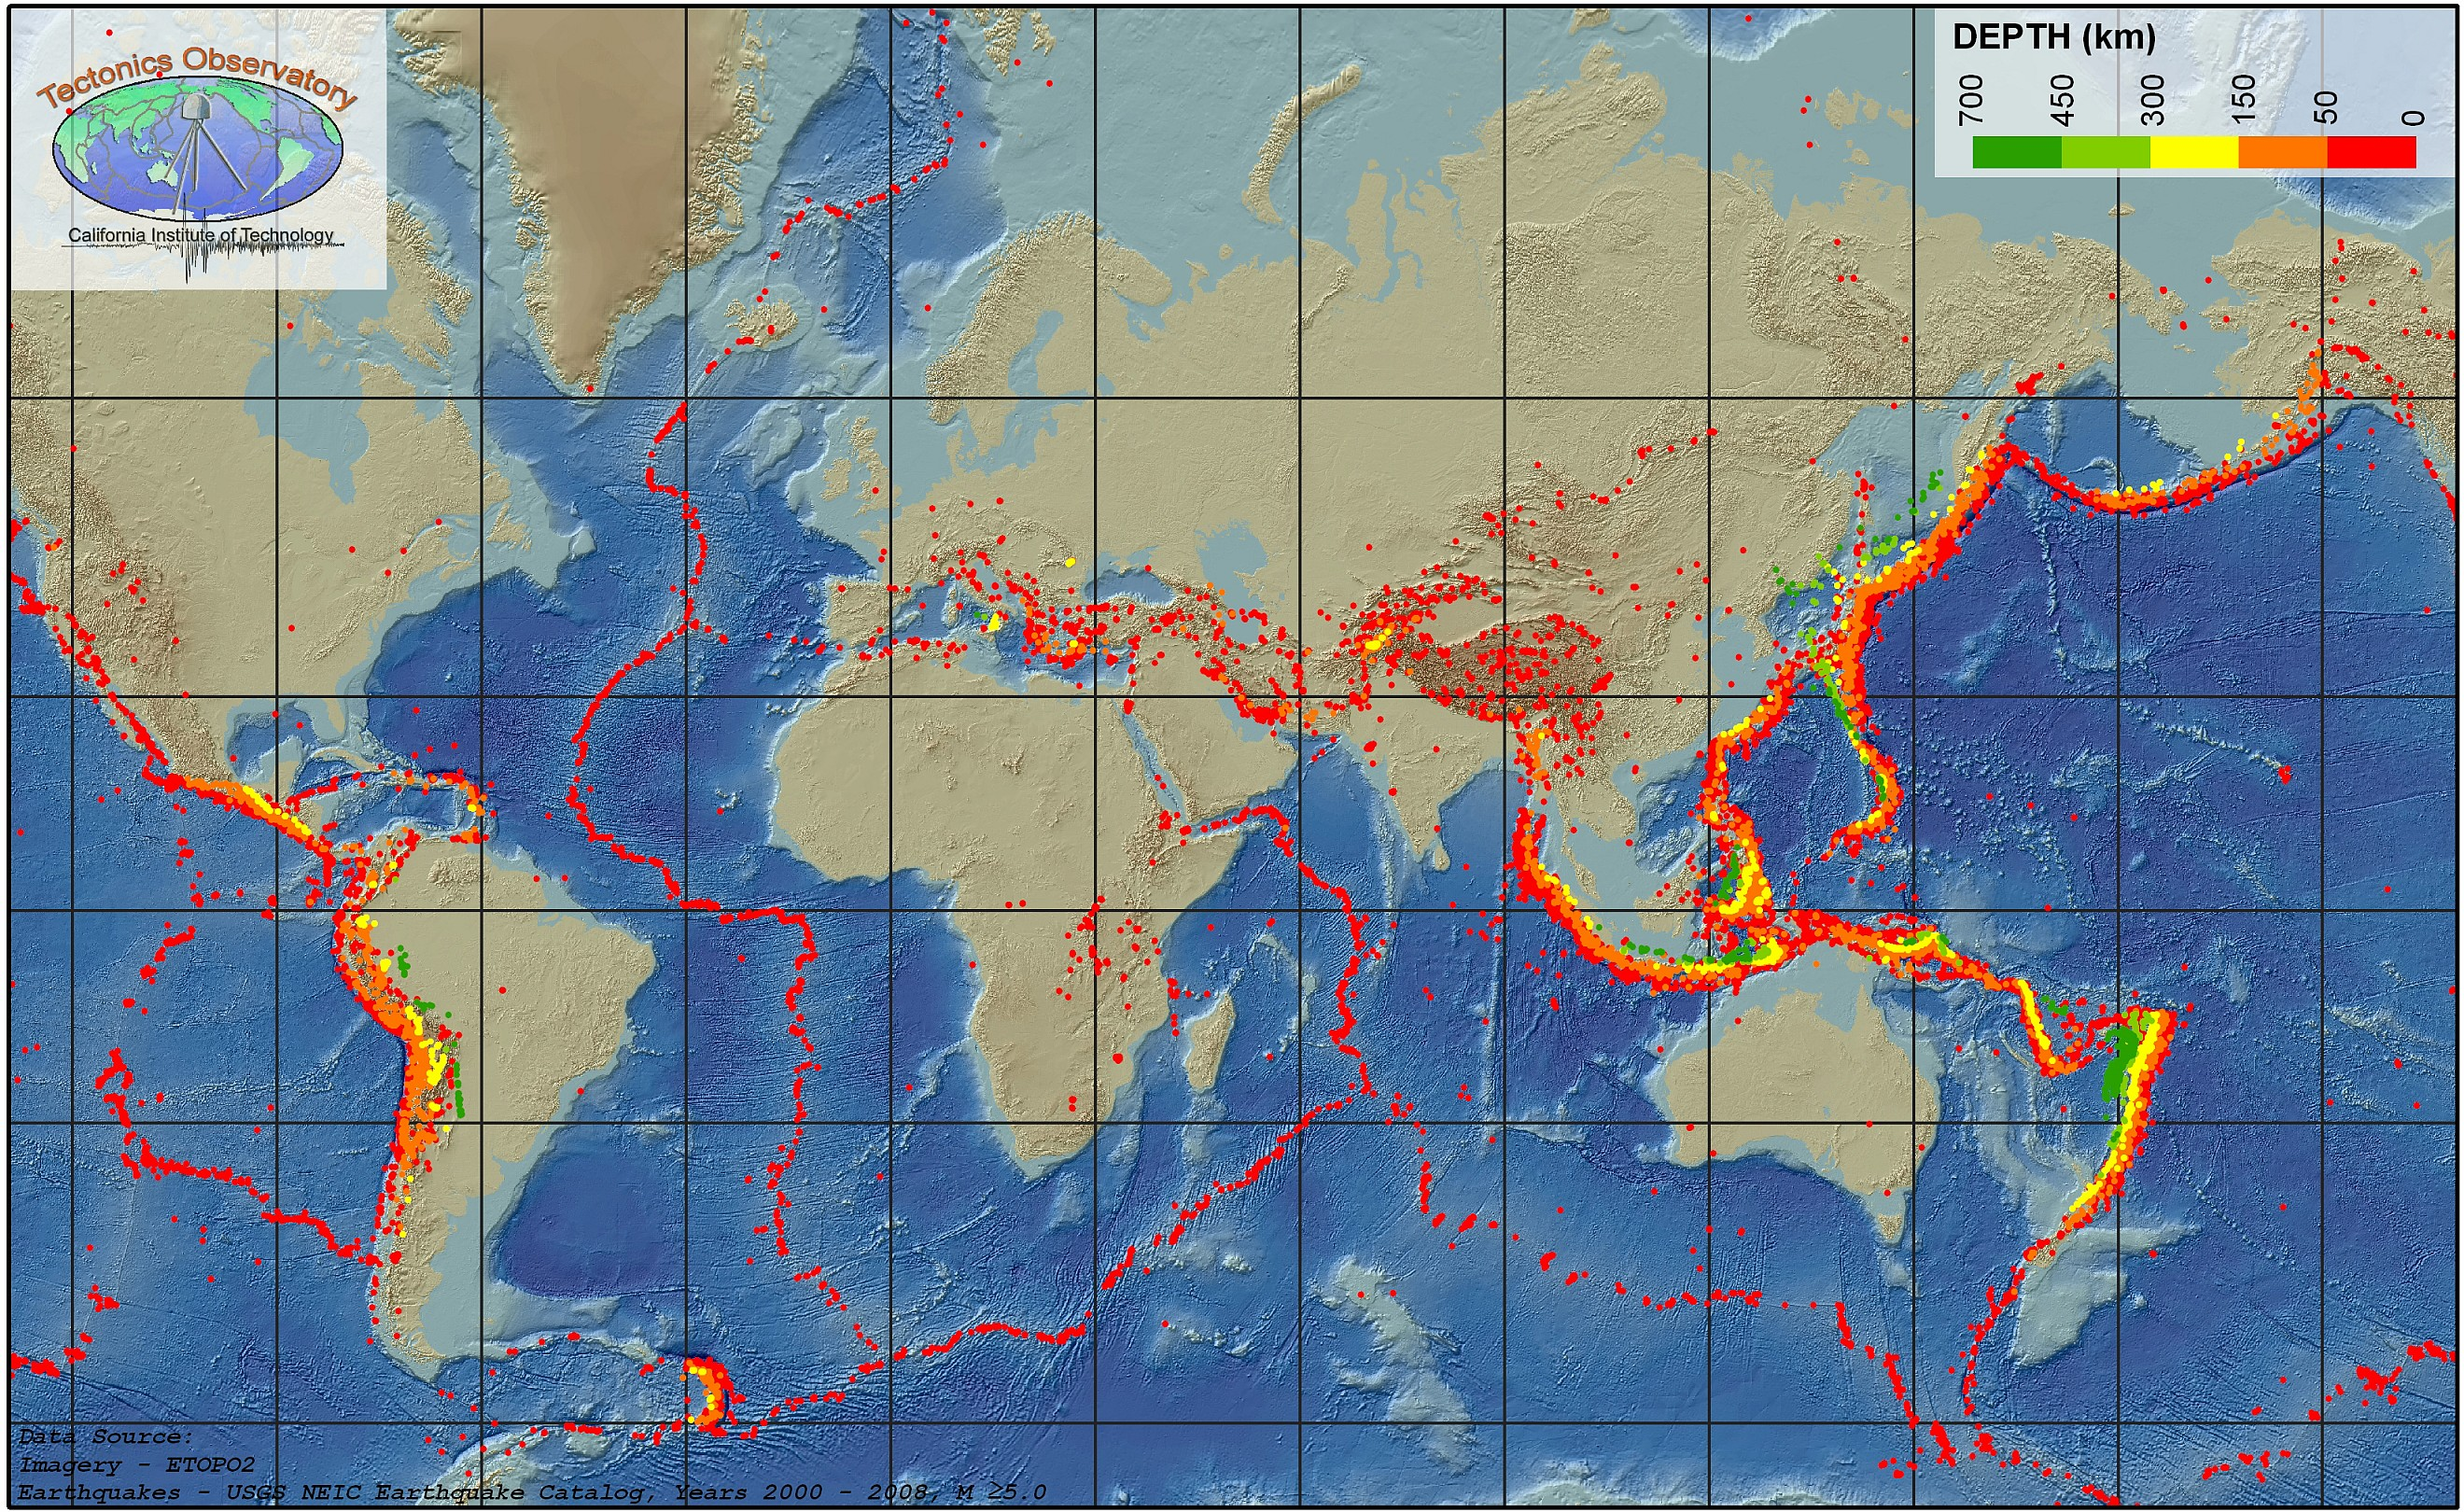
\includegraphics[width=1\linewidth]{obrazky/tectonic/global_seismicity_h}
	\caption{Mapa zemětřesení o magnitudu $>=5$ve světě mezi roky 2000--2008 (Zdroj: Lisa Christiansen, Caltech Tectonics Observatory, \url{https://www.nsf.gov/news/mmg/mmg_disp.jsp?med_id=64691})}
	\label{fig:zemetresenidesky}
\end{figure*}

\subsubsection{Příčiny pohybu litosférických desek}
Příčiny pohybu litosférických desek jsou stále předmětem vědeckého bádání. Je několik mechanismů, kterými je pohyb vysvětlován. Tím hlavním je přítomnost konvekčních proudů v zemském plášti. Tyto proudy vystupují pod středooceánskými hřbety, kde se vychylují do stran a klesají v místech subdukčních zón. Boční pohyb proudů v plášti tak unáší litosférické desky. Další mechanismem je gravitační skluz litosféry. Směrem od středooceánských hřbetů roste její mocnost, což díky gravitaci způsobuje její klouzání směrem k subdukčním zónám. Pohyb strhává astenosféru v přímém kontaktu s litosférickou deskou, což má za následek výstup kompenzačních proudů v místě středooceánských hřbetů. Jako možný mechanismus se uvádí i odtlačování litosférických desek lávou vystupující na povrch v místě středooceánských hřbetů. Jako důležitý mechanismus se ukazuje ponořování oceánské litosféry do astenosféry v zónách subdukce. Stará oceánská litosféra má vyšší hustotu než astenosféra. Část litosférické desky, která se noří do astenosféry až do hloubky cca \SI{700}{\kilo\metre}, tak stahuje její zbylou část sebou. Jelikož mezi litosférou a astenosférou je velký teplotní rozdíl (v hloubce \SI{400}{\kilo\metre} může být litosférická deska až o \SI{1000}{\degreeCelsius} chladnější oproti okolnímu plášti) a litosféra špatně vede teplo, tak vyrovnávání teplot hustoty trvá dlouhou dobu. Pozorování rychlosti pohybu litosférických desek podporuje tento mechanismus. Desky, které mají dlouhé subdukční zóny (jako je např. Pacifická) se pohybují rychleji (\SIrange{60}{90}{\milli\metre\per\rok}) než desky, které nemají tak rozsáhle subdukční zóny (rychlost pod \SI{40}{\milli\metre\per\rok}).

\subsection{Izostáze}
Zjednodušeně lze říct, že litosféra plave na astenosféře podobně jako plave kus dřeva nebo ledová kra na vodní hladině. Aby litosféra dosáhla hydrostatické rovnováhy vzhledem ke své hustotě a tloušťce, dochází u ní k vertikálním pohybům. Pro tento stav rovnováhy byl zaveden právě termín \textbf{izostáze}. Existují dva modely izostáze. \textbf{Prattův model} je založen na rozdílné hustotě různých částí litosféry. To znamená, že jedna sekce litosféry bude výš, než druhá díky své nižší hustotě. \textbf{Airyho model} zase pojednává o rozdílných tloušťkách jednotlivých sekcí litosféry o stejné hustotě. Oba modely se ale mohou kombinovat. Kontinentální litosféra je výš než oceánská, protože má nižší hustotu a zároveň větší mocnost. Výškové rozdíly v rámci kontinentů jsou spojené s rozdíly v mocnosti kontinentální kůry. Vysoká pohoří mají hluboké kořeny z hornin o menší hustotě.
% TODO: \usepackage{graphicx} required
\begin{figure*}[h]
	\centering
	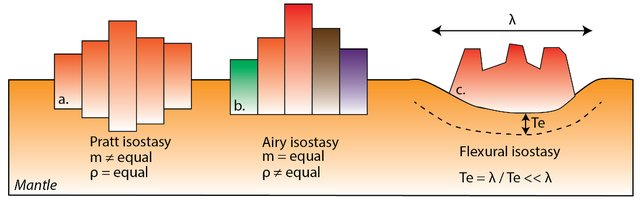
\includegraphics[width=1\linewidth]{obrazky/tectonic/isostasy}
	\caption{Tři typy izostáze. A) Prattův model izostáze b) Airyho model c) Flexurní izostáze způsobena zatížením litosféry např. ledovcem -- glaciizostáze. (Zdroj: \textcite{beniestContinentalRiftingConjugate2017})}
	\label{fig:isostasy}
\end{figure*}

Zvláštním typem izostáze je tzv. \emph{glaciisostáze}. Ledovce během glaciálu svou vahou způsobily prohnutí zemské kůry, což vedlo ke kompenzačnímu výzdvihu v okolí kontinentálních ledovců. Důsledkem zániku ledovce je návrat zemské kůry do rovnovážné polohy. V místech kde zemská kůra byla zatlačena tak dochází ke \emph{glaciisostatickému výzdvihu} (\textit{glaciisostatic rebound}) a naopak k poklesům, kde byla předtím vyzdvižena.
\subsection{Horké skvrny}
Horké skvrny (\textit{hot spots}) jsou specifická místa v zemském tělese, kde je zvýšený tok geotermální energie a magma se dostává k povrchu. Z toho pak pramení vulkanická činnost. Tyto vulkanické oblasti nekopírují okraje litosférických desek. Jelikož se horké skvrny nepohybují, vznikají v důsledku posunu litosférických desek řetězce sopečných ostrovů. Klasickým příkladem je Havajské souostroví (Obr. \ref{fig:hawaiihotspot}).

% TODO: \usepackage{graphicx} required
\begin{figure*}
	\centering
	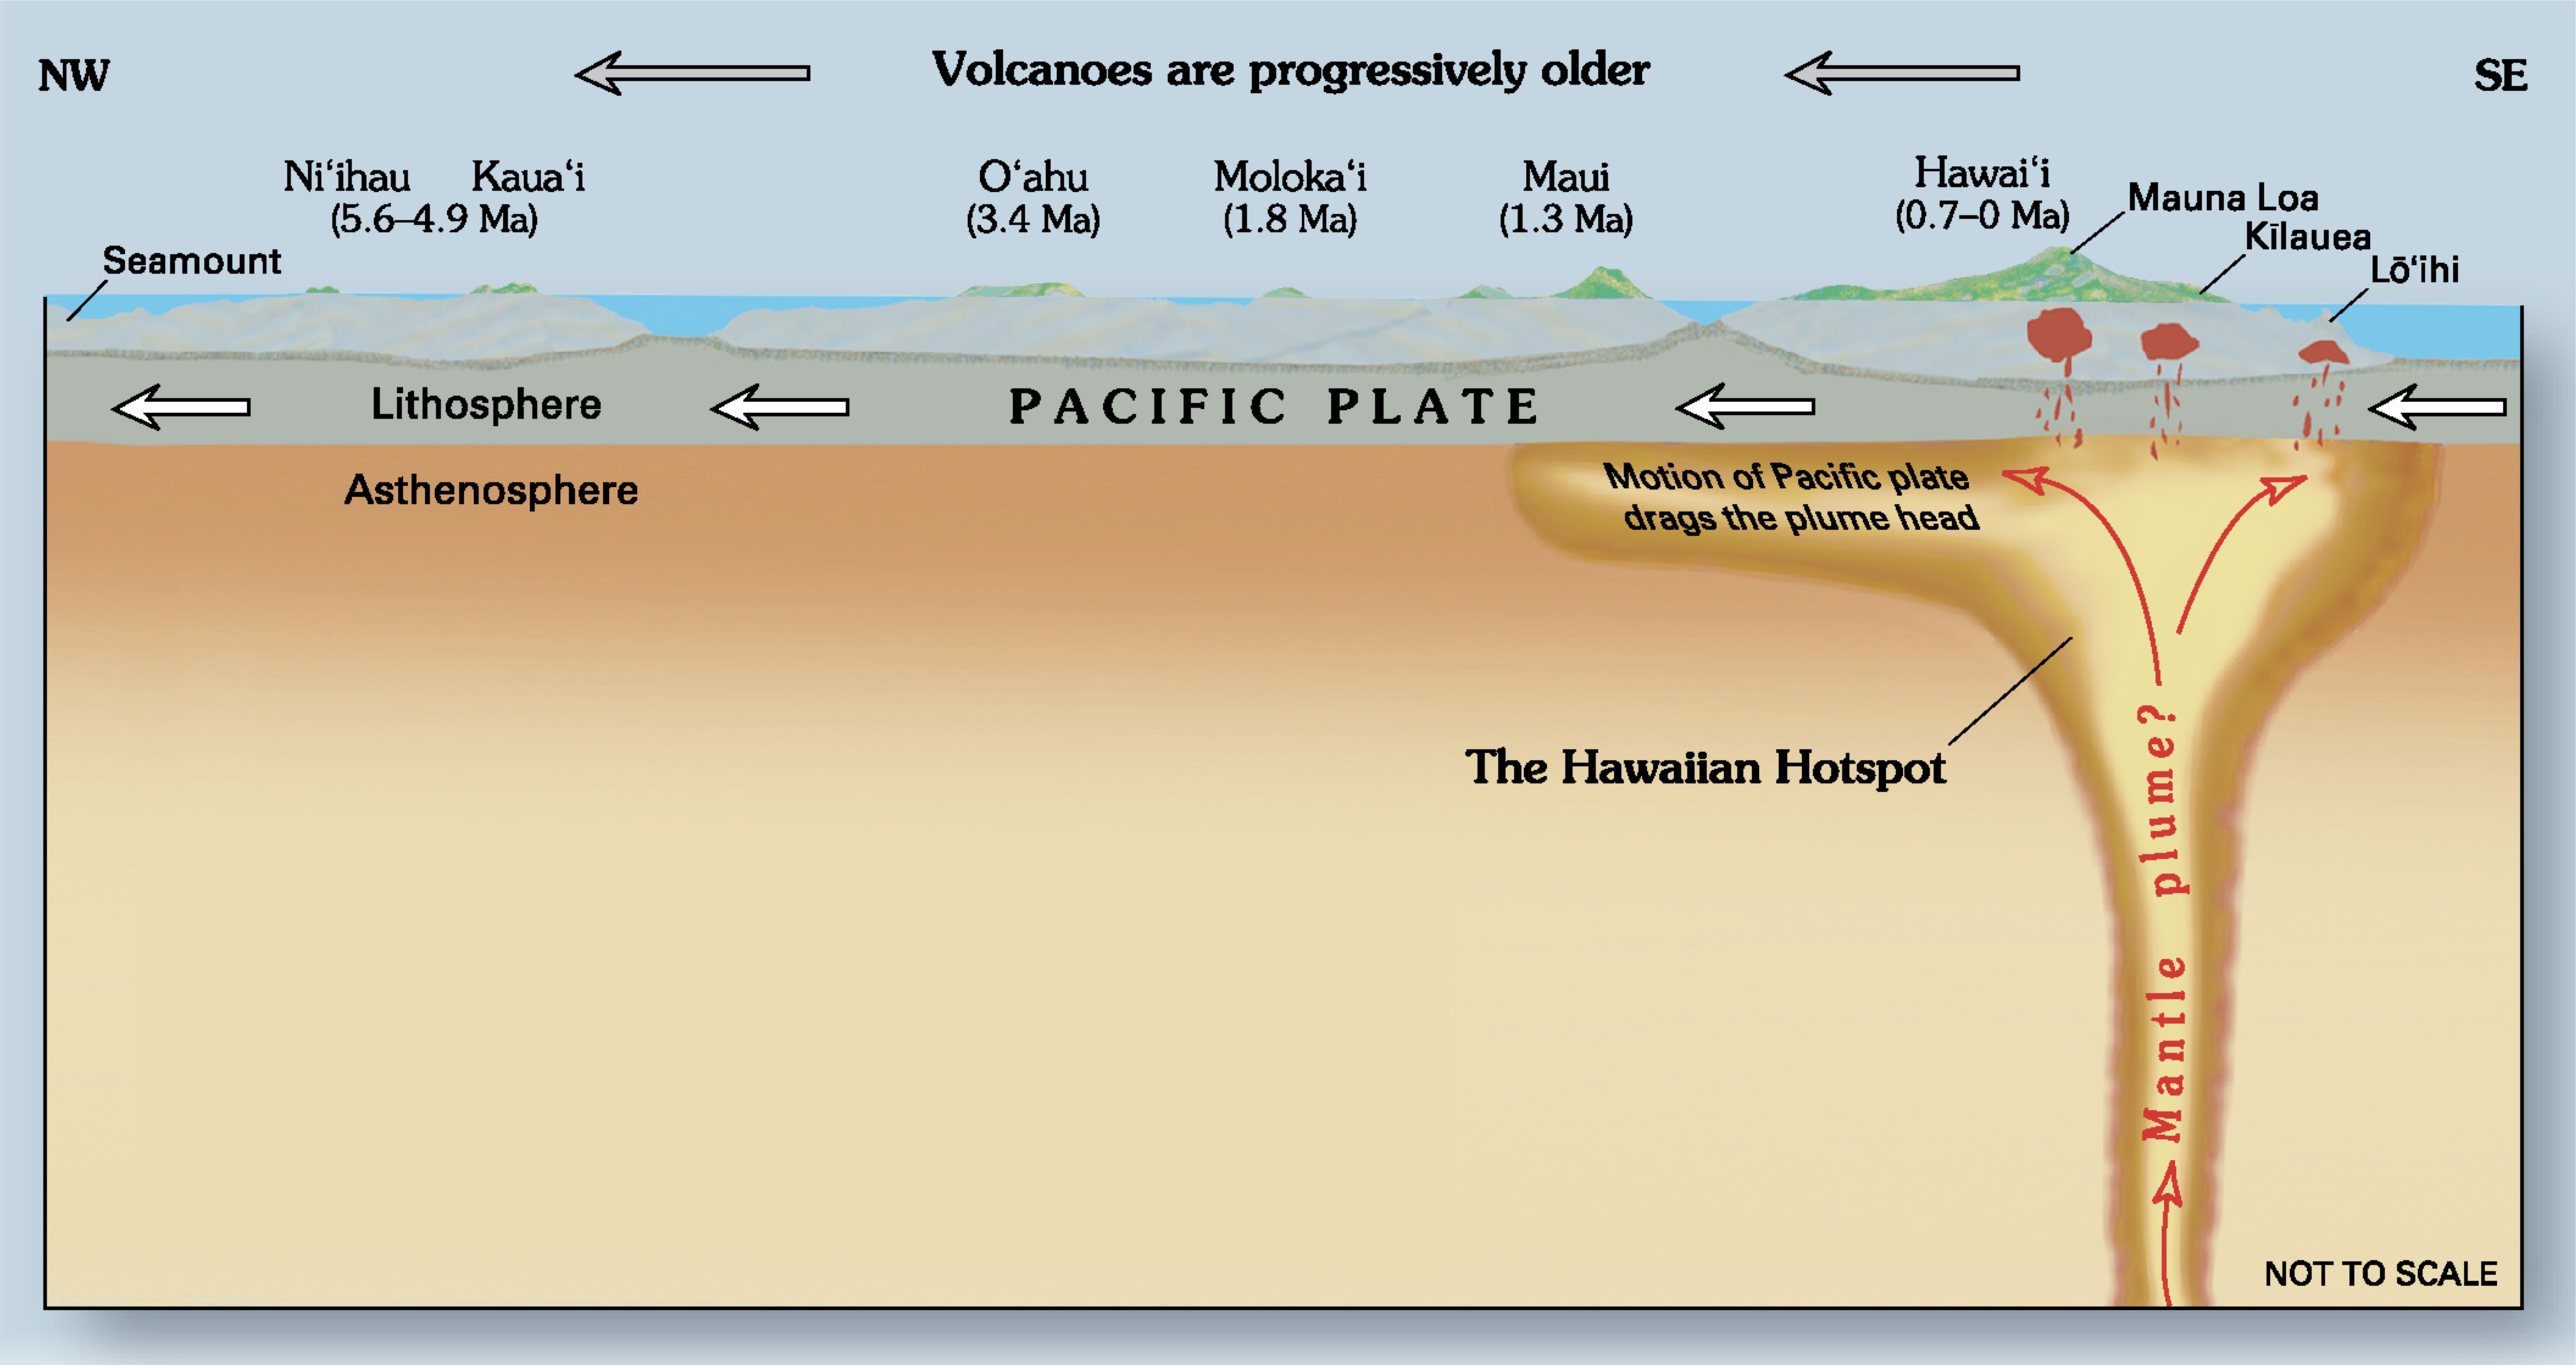
\includegraphics{obrazky/tectonic/Hawaii_hotspot}
	\caption{Diagram zobrazující Havajskou horkou skvrnu (Autor Joel E. Robinson, USGS).}
	\label{fig:hawaiihotspot}
\end{figure*}

\section{Globální geomorfologie}
\subsection{Globální hypsometrie}
Histogram nadmořských výšek (a hloubek) má bimodální charakter. První vrchol odpovídá oceánským pánvím, druhý kontinentálním platformám.

\subsection{Megaformy}
\subsubsection{Formy reliéfu okrajů litosférických desek}
\emph{Konvergentní okraj} je spojen s orogenními pochody. Tedy pochody, při nichž dochází ke vzniku pohoří. Jak již bylo řečeno, na konvergentním okraji se litosférické desky pohybují proti sobě. Můžeme rozlišit dva typy konvergentních okrajů a to \textbf{okraje v rovnovážném stavu} a \textbf{kolizní okraje}. Okraje v rovnovážném stavu jsou takové, kde se oceánská litosférická deska podsouvá jinou oceánskou nebo pevninskou desku. Na rozhraní dvou oceánských desek vzniká \textbf{vulkanický ostrovní oblouk}. Příkladem jsou souostroví v Tichém oceánu. Pokud se oceánská deska podsouvá pod pevninskou, vznikají \textbf{orogénní pásma na okrajích kontinentů} a jedná se o tzv. aktivní okraj kontinentu. Kolizní rozhraní litosférických mají řadu forem v závislosti na podobě jejich okrajů. Prvním příkladem je kolize dvou kontinentů. K tomu dochází v situaci, kdy subdukující deska nese na svém okraji kontinentální kůru. Dochází tak k postupnému přiblížování kontinentů a jejich následné kolizi. To vede ke vzniku vnitrokontinentálních kolizních orogénů. Typickým příkladem takového orogénu jsou Himaláje. Původní subdukční zóna je přeměněna na suturní zónu, kde jsou dva kontinenty do sebe stmeleny. Druhý typ kolize nastává, když oceánská deska nese ostrovní oblouky a subdukuje pod pevninskou desku. Dochází k nasunutí těchto ostrovů na okrajové kontinentální pohoří, které je tak modifikováno. Třetí typ nastává, když původně subdukující oceánská litosférická deska má i svou pevninskou část. Následně dochází ke střetu kontinentu s ostrovním obloukem, vzniká kontinentální okrajový orogén. Následně je subdukce obnovena, ale s opačnou polaritou. Při kolizi ostrovních oblouků a za předpokladu, že nebude subdukován může dojít k uzavření jedné subdukční zóny, případně k obrácení.

\emph{Divergentní okraj} neboli extenzní zóna se vyznačuje vznikem nové zemské kůry. Většina divergentních okrajů se nachází uprostřed oceánů, kde tvoří středooceánské hřbety. V případě pevniny vznikají v místech divergentního okraje rozsáhlé \textbf{kontinentální rifty}. Jedná se o protáhlé sníženiny na povrchu kontinentů. Jsou tvořeny pokleslou krou a bočními, relativně vyzdviženými bloky, které jsou směrem ke dnu riftu omezeny poklesovými zlomy. Rozlišujeme \textbf{aktivní rifting}, který je vyvolán vyklenutím území magmatickým tělesem a \textbf{pasivní rifting}, který je indukován až po průniku magmatu v důsledku ztenčení litosféry. V případě aktivního riftingu existuje nejprve vyklenutí a až posléze se vyvíjí riftové údolí, v případě pasivního riftinngu je tomu naopak. Rift je první fází vývoje tzv. pasivního okraje kontinentu.

\emph{Transformní okraj} může vypadat jako jednoduchá zlomová linie nebo složitá zlomová zóna. U transformních okrajů nedochází zpravidla jen k pohybu podél zlomů, ale dochází k lokalizované kompresi či extenzi. Vznikají tak sníženiny \textit{pullapart basins} respektive transpresní hřbety.

\subsubsection{Formy reliéfu vnitřku kontinentů}
Centrální části kontinentů se skládají z kratonů. \emph{Kraton} je stará a stabilní část zemské kůry. Skládají se ze \emph{štítu} (\textit{shield}), který je tvořen krystalickými horninami (metamorfity, magmatické) komplexně deformovanými. Sedimentární pokryv štítů takřka chybí. Druhou částí kratonu je \emph{platforma} (\textit{platform}). Jedná se o oblast tvořenou mladšími, tektonicky nedeformovanými sedimentárními horninami 

\textbf{Kontinentální pánve} jsou sníženiny (deprese) rozsáhlých rozměrů. Mají plochý reliéf a typická je pro ně velká mocnost sedimentů. Existuje několik mechanismů, kterými mohou vznikat. Jedná se o tektonické poklesy, termickou izostázi v důsledku ochlazování zemské kůry. Dále mohou vznikat zaplňováním iniciální deprese sedimenty. Ty zatěžují zemskou kůru a dochází k dalším poklesům tzn. je tam pozitivní zpětná vazba. Zátěž centra - pokles, snos sedimentů z okolních vyvýšenin a následný kompenzační výzdvih na okrajích.

\begin{figure*}
	\centering
	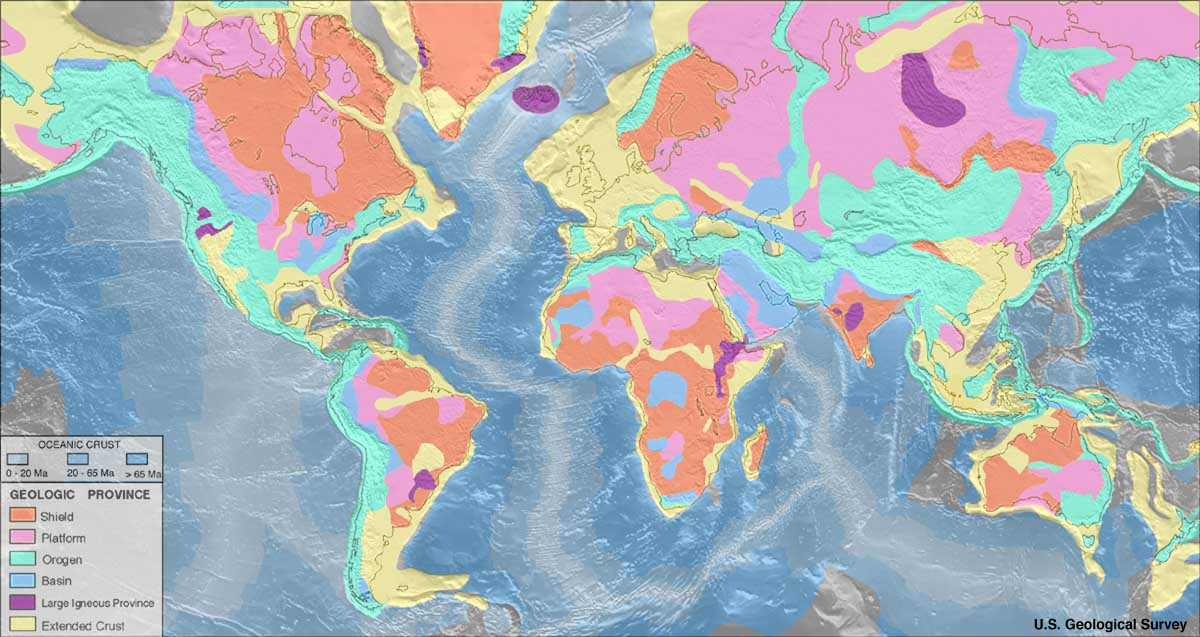
\includegraphics[width=1\linewidth]{obrazky/tectonic/World_geologic_provinces}
	\caption{Mapa geologických provincií (USGS, volné dílo, via Wikimedia Commons)}
	\label{fig:worldgeologicprovinces}
\end{figure*}

%\newpage
%\onecolumn
%\begin{boxotazky}{Kontrolní a klíčové otázky, na které bychom měli znát odpověď}
%	\begin{itemize}
%		\item 
%		\item 
%		
%	\end{itemize}
%\end{boxotazky}
%
%\begin{boxslovnik}{Další klíčové pojmy k zapamatování}
%	aaa & adfasd \\
%	
%\end{boxslovnik}
%\twocolumn